% $Id: template.tex 11 2007-04-03 22:25:53Z jpeltier $

\documentclass{vgtc}                          % final (conference style)
%\documentclass[review]{vgtc}                 % review
%\documentclass[widereview]{vgtc}             % wide-spaced review
%\documentclass[preprint]{vgtc}               % preprint
%\documentclass[electronic]{vgtc}             % electronic version

%% Uncomment one of the lines above depending on where your paper is
%% in the conference process. ``review'' and ``widereview'' are for review
%% submission, ``preprint'' is for pre-publication, and the final version
%% doesn't use a specific qualifier. Further, ``electronic'' includes
%% hyperreferences for more convenient online viewing.

%% Please use one of the ``review'' options in combination with the
%% assigned online id (see below) ONLY if your paper uses a double blind
%% review process. Some conferences, like IEEE Vis and InfoVis, have NOT
%% in the past.

%% Figures should be in CMYK or Grey scale format, otherwise, colour
%% shifting may occur during the printing process.

%% These few lines make a distinction between latex and pdflatex calls and they
%% bring in essential packages for graphics and font handling.
%% Note that due to the \DeclareGraphicsExtensions{} call it is no longer necessary
%% to provide the the path and extension of a graphics file:
%% \includegraphics{diamondrule} is completely sufficient.
%%
\ifpdf%                                % if we use pdflatex
  \pdfoutput=1\relax                   % create PDFs from pdfLaTeX
  \pdfcompresslevel=9                  % PDF Compression
  \pdfoptionpdfminorversion=7          % create PDF 1.7
  \ExecuteOptions{pdftex}
  \usepackage{graphicx}                % allow us to embed graphics files
  \DeclareGraphicsExtensions{.pdf,.png,.jpg,.jpeg} % for pdflatex we expect .pdf, .png, or .jpg files
\else%                                 % else we use pure latex
  \ExecuteOptions{dvips}
  \usepackage{graphicx}                % allow us to embed graphics files
  \DeclareGraphicsExtensions{.eps}     % for pure latex we expect eps files
\fi%

%% it is recomended to use ``\autoref{sec:bla}'' instead of ``Fig.~\ref{sec:bla}''
\graphicspath{{figures/}{pictures/}{images/}{./}} % where to search for the images

\usepackage{microtype}                 % use micro-typography (slightly more compact, better to read)
\PassOptionsToPackage{warn}{textcomp}  % to address font issues with \textrightarrow
\usepackage{textcomp}                  % use better special symbols
\usepackage{mathptmx}                  % use matching math font
\usepackage{times}                     % we use Times as the main font
\renewcommand*\ttdefault{txtt}         % a nicer typewriter font
\usepackage{cite}                      % needed to automatically sort the references
\usepackage{tabu}                      % only used for the table example
\usepackage{booktabs}                  % only used for the table example
%% We encourage the use of mathptmx for consistent usage of times font
%% throughout the proceedings. However, if you encounter conflicts
%% with other math-related packages, you may want to disable it.

\usepackage{caption}
\captionsetup[table]{skip=10pt}
\usepackage{tabularx}
\usepackage{todonotes} %TODO: Remove after all TODO's are gone

%% If you are submitting a paper to a conference for review with a double
%% blind reviewing process, please replace the value ``0'' below with your
%% OnlineID. Otherwise, you may safely leave it at ``0''.
\onlineid{0}

%% declare the category of your paper, only shown in review mode
\vgtccategory{Research}

%% allow for this line if you want the electronic option to work properly
\vgtcinsertpkg

%% In preprint mode you may define your own headline.
%\preprinttext{To appear in an IEEE VGTC sponsored conference.}

%% Paper title.

\title{Type Visualization for R}

%% This is how authors are specified in the conference style

%% Author and Affiliation (single author).
%%\author{Roy G. Biv\thanks{e-mail: roy.g.biv@aol.com}}
%%\affiliation{\scriptsize Allied Widgets Research}

%% Author and Affiliation (multiple authors with single affiliations).
%%\author{Roy G. Biv\thanks{e-mail: roy.g.biv@aol.com} %
%%\and Ed Grimley\thanks{e-mail:ed.grimley@aol.com} %
%%\and Martha Stewart\thanks{e-mail:martha.stewart@marthastewart.com}}
%%\affiliation{\scriptsize Martha Stewart Enterprises \\ Microsoft Research}

%% Author and Affiliation (multiple authors with multiple affiliations)
\author{Roy G. Biv\thanks{roy.g.biv@aol.com}\\ %
        \scriptsize Starbucks Research %
\and Ed Grimley\thanks{ed.grimley@aol.com}\\ %
     \scriptsize Grimley Widgets, Inc. %
\and Martha Stewart\thanks{martha.stewart@marthastewart.com}\\ %
     \parbox{1.4in}{\scriptsize \centering Martha Stewart Enterprises \\ Microsoft Research}}

%% A teaser figure can be included as follows, but is not recommended since
%% the space is now taken up by a full width abstract.
%\teaser{
%  \includegraphics[width=1.5in]{sample.eps}
%  \caption{Lookit! Lookit!}
%}

%% Abstract section.
\abstract{
  Data-driven approaches to programming language design are uncommon.
  Despite the availability of large code repositories, distilling useful
  information from programs remain difficult. Important dimensions of
  code, like run-time type data, are inscrutable without appropriate tools.
  We built {\sc TypeVis} to explore and analyze run-time types in
  the R programming language by means of visualization.
  Our system focuses on understanding and comparing the type signatures of
  function calls across the R ecosystem.
  {\sc TypeVis} uses flows to intuitively represent categorical
  and numerical aspects of type signatures.
  Insights derived from our visualization are aimed at informing
  language design decisions---specifically of a gradual type system
  currently being developed for R.

  \todo{Fill in keywords below.}
} % end of abstract

%% ACM Computing Classification System (CCS).
%% See <http://www.acm.org/about/class> for details.
%% We recommend the 2012 system <http://www.acm.org/about/class/class/2012>
%% For the 2012 system use the ``\CCScatTwelve'' which command takes four arguments.
%% The 1998 system <http://www.acm.org/about/class/class/2012> is still possible
%% For the 1998 system use the ``\CCScat'' which command takes four arguments.
%% In both cases the last two arguments (1998) or last three (2012) can be empty.

\CCScatlist{
%  \CCScatTwelve{Human-centered computing}{Visu\-al\-iza\-tion}{Visu\-al\-iza\-tion techniques}{Treemaps};%  \CCScatTwelve{Human-centered computing}{Visu\-al\-iza\-tion}{Visualization design and evaluation methods}{}
}

%\CCScatlist{
  %\CCScat{H.5.2}{User Interfaces}{User Interfaces}{Graphical user interfaces (GUI)}{};
  %\CCScat{H.5.m}{Information Interfaces and Presentation}{Miscellaneous}{}{}
%}

%% Copyright space is enabled by default as required by guidelines.
%% It is disabled by the 'review' option or via the following command:
% \nocopyrightspace

%%%%%%%%%%%%%%%%%%%%%%%%%%%%%%%%%%%%%%%%%%%%%%%%%%%%%%%%%%%%%%%%
%%%%%%%%%%%%%%%%%%%%%% START OF THE PAPER %%%%%%%%%%%%%%%%%%%%%%
%%%%%%%%%%%%%%%%%%%%%%%%%%%%%%%%%%%%%%%%%%%%%%%%%%%%%%%%%%%%%%%%%

\begin{document}

%% The ``\maketitle'' command must be the first command after the
%% ``\begin{document}'' command. It prepares and prints the title block.

%% the only exception to this rule is the \firstsection command
\firstsection{Introduction}

\maketitle

%% \section{Introduction} %for journal use above \firstsection{..} instead

Programming languages commonly evolve by decree. The designer
decides that a new feature is necessary or that a past feature was
ill-conceived, and thus the language and its users move forward.
Sometimes these changes are the result of rigorous theory
or the product of community feedback. However, language design is
rarely informed by empirical data about how programs are actually
written in practice.

For a popular language, data collection is no challenge. Vast
quantities of publicly available code are hosted on open source
repositories like Github and language-specific package servers like npm.
Rather, the difficulty lies with analyzing and interpreting the data
at hand. Code is complex and highly structured. Simple
semantically-ignorant metrics like ``lines of code''
carry little significance.

To analyze one aspect of programming languages, we built {\sc TypeVis},
an interactive visualization of run-time types for the language R.
{\sc TypeVis} builds on a dataset of concrete execution traces
over the most widely used libraries in the R ecosystem.
Our visualization supports three broad tasks:
filtering the dataset down to a digestible subset,
understanding the types of function arguments and returns,
and comparing across different functions.
For filtering, {\sc TypeVis} uses the treemap idiom
to convey the relative scale of different packages.
Once a specific function is selected,
type signatures are represented as flows over types
where the width of the flow is proportional to frequency.
These flows can be readily compared within the same function,
or across different functions.

Tasks enabled by {\sc TypeVis} can assist language designers
during many phases of development.
For example, exploratory data analysis can weed out designs that
are incompatible with existing programs.
In particular, the visualization is built to answer questions
relevant to gradual type system development.
Supplemental material, including the data and source code of
{\sc TypeVis}, is freely available: \todo{Fill with archival link}

%%

\section{Background and Related Work}

% R background

% gradual typing background

% vis papers

\todo{
  We need to take a closer look at the papers we cite.
}

%%

\section{Data and Collection}

\todo{Alexi's paper says 412, but I see more packages in our data.}

The data consists of traces from 412 packages
containing over $760,000$ lines of R code
and $534,000$ lines of native code.
All libraries were obtained from CRAN,
the most popular R code repository.
Packages hosted on CRAN must satisfy certain criteria
to ensure they are high quality.
Additionally, the subset of 412 packages chosen here
all had code coverage above 65\%.

Each execution trace was recorded by running
the test, example, and vignette code of each package.
A vignette is a form of documentation that weaves
together prose and executable code.
An execution trace is a list of ``raw'' type signatures
containing, among other attributes, the function name
and type tags for each argument and return value.
Our dataset consists of a table of traces
that have been processed to reduce some fields.
Traces were generated via a dynamic analysis
that instruments the R virtual machine with hooks
that intercept the required data at run-time.

While {\sc TypeVis} has only been run with
data from R execution traces, the architecture is not
limited to R.
Any dynamically typed language with the right run-time
hooks could generate data for the tool.
As long as execution trace information is adheres to
the same database schema, {\sc TypeVis} will
work properly without any modifications.

%%

\section{Task Abstraction}

\bgroup
\def\arraystretch{1.75}
\begin{table*}
  \centering
  \begin{tabularx}{\linewidth}{c|c|c|X}
    Domain Goals & Search Task & Query Task & \multicolumn{1}{c}{Abstract Task Description} \\
    \hline
    Find Function & Locate & Identify & Finding a function is a location task, where the target function is known, but its location within the package hierarchy is not. Once the desired function is found, a user must be able to identify data of interest. \\

    Determine Types & Browse & Identify & Determining types is a browse task, where the target type signature is unknown, but the location of the function of interest is known. While browsing, a user must be able to identify the frequencies of particular type signatures.\\

    Compare Signatures & Lookup & Compare & Comparing type signatures is a lookup task where both target type signatures have already been located. A user must be able to discern how often a signature is used compared to another, both within a function and across different functions.\\
  \end{tabularx}
  \caption{Domain goals and their mid-level and low-level task abstractions.}
  \label{tab:tasks}
\end{table*}
\egroup

We interviewed the primary researcher developing R's gradual type system
to inventory relevant domain-specific tasks.
Additionally, we sought feedback throughout the creation of {\sc TypeVis}
to ensure it was adequately satisfying requirements.
The domain-specific goals can be reduced to:

\begin{enumerate}
\item {\bf Find Function.} Quickly search for a particular function and identify basic information. This includes how often the function is called and which package contains it.
\item {\bf Determine Types.} Given a specific function, determine the argument and return types of the function. Additionally, identify the frequency of a type signature. A user should be able to infer, for example, if the function is polymorphic or if it's a predicate.
\item {\bf Compare Signatures.} Compare the occurrence of type signatures within a specific function, but also across many different ones. Users must be able to isolate individual signatures and see them in the context of other signatures and functions.
\end{enumerate}

These goals can be classified using an abstract task analysis framework.
See table~\ref{tab:tasks} for a categorization of these domain tasks
into Munzner's mid-level and low-level abstract task taxonomy. \todo{Cite Munzner}

%%

\section{Design and Implementation}

{\sc TypeVis} is an interactive web-based visualization
that permits real-time exploration,
even with large datasets.
The default dataset contains over a million rows
based on the analysis of almost five hundred
different R packages.
Figure~\ref{fig:typevis} displays
the heart of {\sc TypeVis}
in its initial configuration.
Most aspects of the system can be tweaked
by a user if desired.

\subsection{Function Filtering}

The right-hand panel of figure~\ref{fig:typevis}
contains three elements: a search bar,
a package treemap,
and a function treemap.
All three are linked.
Selecting a package
in the top treemap will immediately narrow the
bottom view to only functions available in that package.
Additionally, entering a function name in the search
will select it in the function treemap.

These different components support different modes of search.
If a user has a specific function in mind,
the search bar supports autocomplete
that can quickly select a function among thousands.
However, if one wants to browse
all available functions and packages,
the treemap view is more applicable.
Nodes in the bottom treemap convey the log-scaled
frequency of function calls,
and correspondingly the top treemap
is scaled based on invocations
of functions defined in that package.
Log-scaling and pagination keep
elements of the treemap legible,
even if absolute size differences are significant.

If configured, {\sc TypeVis} allows for multiple function selection.
Both the {\tt length.unit} and {\tt valid.unit} functions
from the {\tt grid} package are selected in figure~\ref{fig:typevis}.
These functions are rendered simultaneously in the type flow
panel, allowing one to make comparisons between them.

\subsection{Types as Flows}

Prominently featured as the center visualization,
a Sankey diagram encodes type signatures of the selected
functions as flows.
Flows begin at nodes labeling a function,
curve across each argument type in order,
and terminate at the return type.
Widths are proportional to how many times a function
is called with that signature during analysis.
Flow segments are filled with a hue-varying color scale,
based on the type where the segment ends.
Beneath each node label is an approximate count.
If the node represents a function, then the
number is how many times the function was invoked.
If the node represents a type, then the
number is how often a value of that type
at that argument position was recorded during analysis.

For example, in figure~\ref{fig:typevis},
the {\tt length.unit} function is called with
two different type signatures at run-time.
Most frequently, the function is used with the
signature {\tt double $\to$ integer},
but a substantial fraction of the time it is
used as {\tt double[] $\to$ integer}.
Here, {\tt double[]} stands for an array of
doubles with arbitrary dimension.

Interactivity significantly augments the
usability of the Sankey visualization.
Hovering over a flow will highlight the
entire path of the flow
and will fade other functions
into the background.
When displaying many flows at the same time,
highlighting becomes especially critical
for user comprehension.
Additional quantitative information
about the flow is also supplied
while hovering.
Clicking a flow will focus on that function
only, filtering away all others.

Flow layout is a critical consideration
for a sufficiently legible visualization.
Figure~\ref{fig:decross} exemplifies what
happens if flow layout is not adequately handled.
The top layout was generated without any
flow decrossing algorithm,
while the bottom layout does
apply decrossing.
Even with highlighting,
the utility of the visualization is vastly
reduced without some decrossing effort.
To maintain real-time performance,
we use two different decrossing methods.
First, the system attempts to construct
a layout with the globally optimal
minimum amount of flow crossing by
solving a mixed-integer linear program.
Unfortunately, for even moderately
sized graphs this can take too long to compute.
Therefore, after about $1$ second
the optimal algorithm is terminated
if it has not finished, and a faster
algorithm that only locally minimizes crossing
between layers computes the layout.

\subsection{Technical Details}

Since the amount of data that a user may query is large,
the application consists of both a frontend and a backend.

On the frontend, state management, interactivity,
and DOM manipulation is all done within the Vue framework.
This is in contrast with many web-based visualizations
that use D3 for DOM manipulation.
We chose this setup because of the many different
individual components whose state must be kept
sychronized.
This includes not only the visualizations, but also
user interface elements like the autocomplete search bar.
In our experience, Vue's model of reactivity is
more successful at maintaining consistency across the
entire system than using D3 and vanilla JavaScript.
While {\sc TypeVis} does not use D3 for DOM manipulation,
it still does use D3 for other visualization-related
computations.

Our backend is a Node.js application that serves
JSON in a standard REST-style architecture.
Data is stored in a SQLite database that has been
indexed to achieve lookups as fast as possible.
To avoid execessive memory consumption and speed up computations,
clients query data from the server on an as-needed basis.
Thus, a stable network connection is required for
real-time interaction.

\begin{figure*}
 \centering
 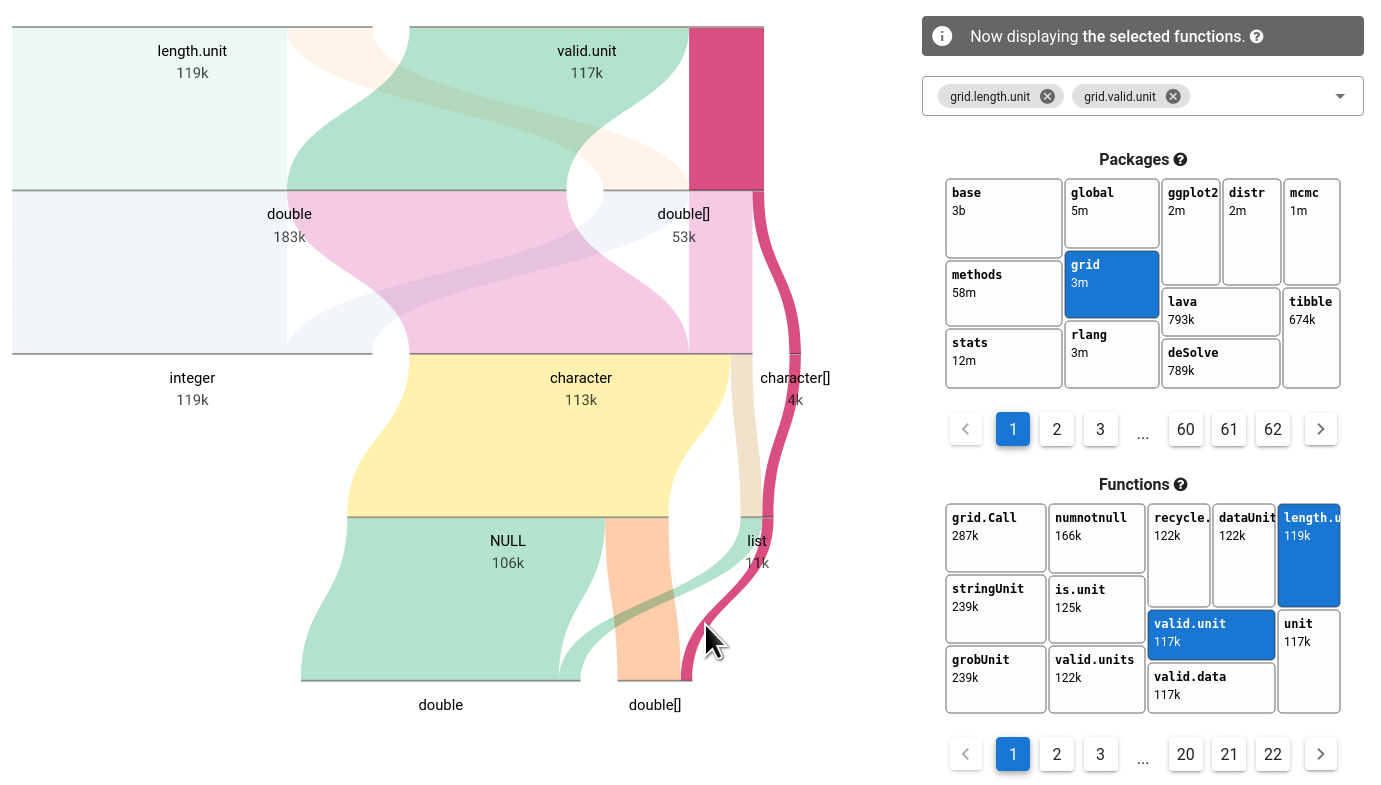
\includegraphics[width=\linewidth]{img/typevis.png}
 \caption{The main view of {\sc TypeVis}, with type flows on the left and the package hierarchy on the right.}
 \label{fig:typevis}
\end{figure*}

\begin{figure}[tb]
 \centering
 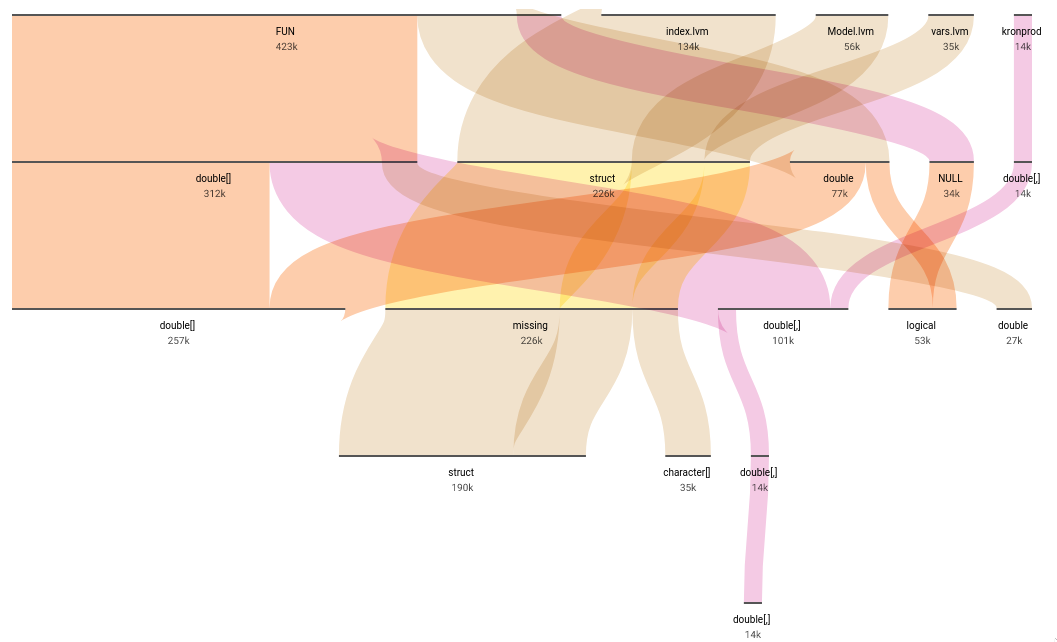
\includegraphics[width=\columnwidth]{img/no_decross.png}
 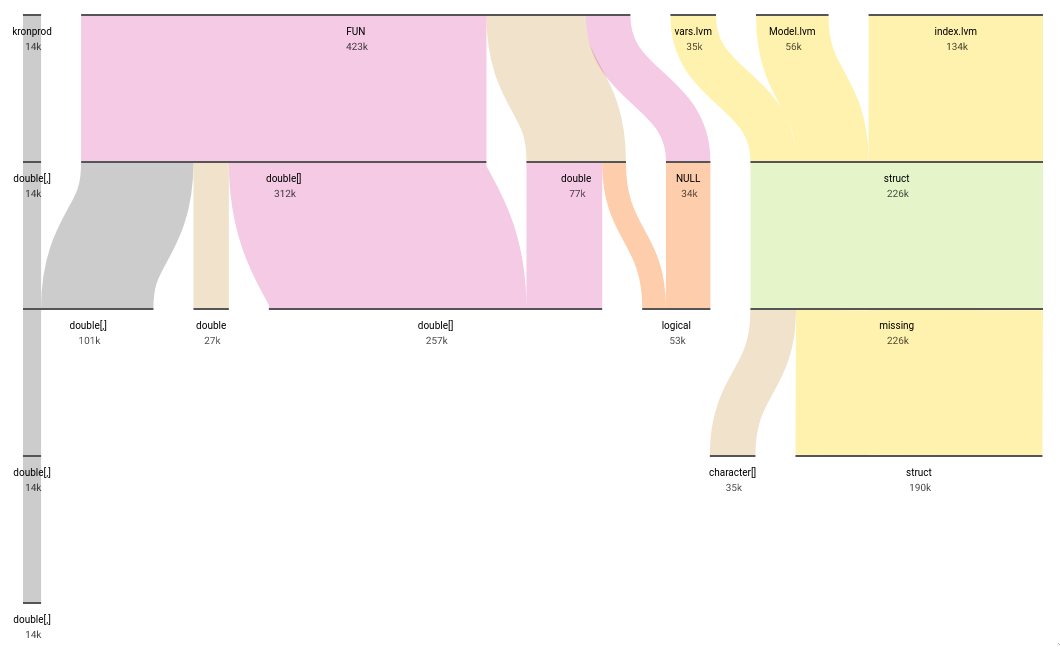
\includegraphics[width=\columnwidth]{img/decross.png}
 \caption{Comparison of type flows without decrossing (above) and with decrossing (below).}
 \label{fig:decross}
\end{figure}

%%

\section{Limitations and Future Work}

{\sc TypeVis} suffers from a number of shortcomings
and does not fully address the entire range of possible tasks
a language designer may need to perform.

In particular, R supports a wide range of data types
including types that contain dimensionality information.
For example, an R array may have type {\tt integer[3]}
indicating that it is an array of length $3$.
This will get compressed down into a single array
type labeled {\tt integer[]}.
Reducing the number of types can make the visualization
more understandable---at the expensive of losing some
precision in type information.
Ideally a user would be able to interactively tune
the level of type granularity based on their interest
in a specific property.
Such a feature would be especially helpful for R
since values can come attached with relevant additional
data such as the dynamic dispatch method
or user-specified metadata.

Filtering is an central mechanism in the system,
but it also comes at a cost.
If one has a specific function or several functions
in mind, then {\sc TypeVis} provides a useful
local view of that type information.
However, it does not support any kind of global
view of type information across a large amount of
functions. When the number of flows or nodes
becomes too great, the visualization will start
paginating, making comparisons over large amounts
of data impossible.
Aggregation and summarization would be key to
making a global view of the data feasible---that
remains future work.

%%

\section{Conclusion}

% other dynamic languages

% other featuers not just types

% general philosophy not just about types
% vis has role to play in language design

\todo{Write.}

\acknowledgments{
  The authors wish to thank A, B, and C. This work was supported in part by
  a grant from XYZ.
}

\bibliographystyle{abbrv-doi}

\bibliography{main}
\end{document}
